\documentclass[twocolumn,amsmath,amssymb,showpacs,prl,superscriptaddress]{revtex4-1} %,preprint,jcp,nofootinbib

\bibstyle{apsrev}
\usepackage{bm}%
\usepackage{graphicx}
\usepackage{tikz}
\usepackage{color}
\usepackage{xcolor}
\usepackage{physics}
\usepackage[colorlinks=true,linkcolor=blue]{hyperref}%
\expandafter\ifx\csname package@font\endcsname\relax\else
 \expandafter\expandafter
 \expandafter\usepackage
 \expandafter\expandafter
 \expandafter{\csname package@font\endcsname}%
\fi
\hyphenation{title}
\newcommand{\JH}[1]{\textcolor{blue}{ JH: #1}}
\newcommand{\REV}[1]{\textcolor{red}{#1}}
%\newcommand{\REV}[1]{#1}


\begin{document}

\definecolor{pyblue}{HTML}{1F77B4}
\definecolor{pyorange}{HTML}{FF7F0C}
\definecolor{pygreen}{HTML}{2CA02C}
\definecolor{pyred}{HTML}{D62728}
\definecolor{jlblue}{rgb}{0.0,0.6056031611752245,0.9786801175696073}
\definecolor{jlorange}{rgb}{0.8888735002725198,0.43564919034818994,0.2781229361419438}
\definecolor{jlgreen}{rgb}{0.2422242978521988,0.6432750931576305,0.3044486515341153}
\definecolor{jlviolet}{rgb}{0.7644401754934356,0.4441117794687767,0.8242975359232758}
\newcommand*\Diff[1]{\mathop{}\!\mathrm{d^#1}}

\title{Controlling the dewetting morphologies of thin liquid films by switchable substrates}

\author{S. Zitz}
\email{zitz@ruc.dk}
 %Changed order: Work done while Stefan worked in Nuremberg
 \affiliation{Helmholtz Institute Erlangen-N\"urnberg for Renewable Energy,\\
  Forschungszentrum J\"ulich,
  F\"urther Strasse 248, 90429 N\"urnberg, Germany}%
  \affiliation{Department of Chemical and Biological Engineering, Friedrich-Alexander-Universit\"at Erlangen-N\"urnberg, F\"{u}rther Stra{\ss}e 248, 90429 N\"{u}rnberg, Germany}
  \affiliation{IMFUFA, Department of Science and Environment,\\ 
Roskilde University, Postbox 260, DK-4000 Roskilde, Denmark}%
\author{A. Scagliarini}%
\email{andrea.scagliarini@cnr.it}
 \affiliation{Institute for Applied Mathematics "M. Picone" (IAC), 
Consiglio Nazionale delle Ricerche (CNR),\\
Via dei Taurini 19, 00185 Rome, Italy}%
\affiliation{INFN, sezione Roma ``Tor Vergata'', via della Ricerca Scientifica 1, 00133 Rome, Italy}
\author{J. Harting}
\email{j.harting@fz-juelich.de}
 \affiliation{Helmholtz Institute Erlangen-N\"urnberg for Renewable Energy,\\
  Forschungszentrum J\"ulich,
  F\"urther Strasse 248, 90429 N\"urnberg, Germany}%
 \affiliation{Department of Chemical and Biological Engineering and Department of Physics, Friedrich-Alexander-Universit\"at Erlangen-N\"urnberg, F\"{u}rther Stra{\ss}e 248, 90429 N\"{u}rnberg, Germany}
\date{\today}

\begin{abstract}
\noindent Switchable and adaptive substrates emerged as valuable tools for controlling wetting and actuation of droplet motion. Here, we report a computational study of the dynamics of an unstable thin liquid film deposited on a switchable substrate, modeled with a space and time varying contact angle.
With a static pattern, all fluid is drained into droplets located around contact angle minima, whereas for a sufficiently large rate of wettability variation a state consisting of metastable rivulets is observed. 
A criterion discriminating whether rivulets occur or not is identified in terms of a single dimensionless parameter.
Finally, we show and explain theoretically how the film rupture times, droplet shape and rivulet life time depend on the pattern wavelength and speed.  
\end{abstract}

\maketitle

\newcommand{\ts}{\textsuperscript}

\noindent {\it Introduction}. Wet surfaces and droplets are part of our every-day experience and of numerous industrial processes including coating, tribology, painting and printing, to name but a few~\cite{gross1980fluid,szeri2010fluid,doi:10.1146/annurev.fluid.31.1.347,DASILVASOBRINHO19991204,singh2010inkjet,Wijshoff2010}. 
Moreover, the continuously growing interest for lab-on-a-chip devices~\cite{C6LC00387G,Focke} as well as for printable electronics or printable photovoltaics~\cite{Luechinger_2008,RH22}, whose efficiency relies crucially on a precise control of material deposition upon (de-)wetting of liquid films, drew the attention to applications where the substrate is adaptive or switchable, i.e. it is not inert but responds dynamically to external stimuli or to the evolution of the coating liquid film itself~\cite{ButtEtAl_Langmuir2018}. 
Several realizations of switchable and adaptive substrates have been proposed~\cite{XiCSR2010}, involving smart materials such as polymer brushes~\cite{CohenStuartEtAl_NatMat2010}, thermal-responsive hydrogels~\cite{ChenEtAl_SM2010}, light-responsive molecules and microstructures~\cite{IchimuraEtAl_Science2000} or processes such as electrowetting~\cite{MugeleEtAl_JPCM2005}.
Probably the simplest, yet non-trivial, modelling of a switchable substrate can be realized by a space and time dependent wettability pattern~\cite{GrawitterStark1}. 
While a consistent body of theoretical/computational work was devoted to processes on static heterogeneous substrates, the time dependent case is still almost unexplored, with few exceptions focusing on single droplet spreading and sliding~\cite{GrawitterStark1,GrawitterStark2,ThieleHartmann} or limited to analysing the linear regime~\cite{suman2006dynamics}.

Here, we study by means of numerical simulations the full dewetting dynamics of a thin liquid film deposited on a substrate with a time varying wettability pattern, from rupture to the long time morphology. 
We identify two regimes where the rupture times grow with the pattern wavelength either linearly (on a static pattern) or attain a constant value (in the time dependent case), for short wavelengths, and approach a quadratic law as the wavelength increases. These observations are then explained theoretically.
We show that, by tuning the rate of change (the ``speed'') of the underlying pattern, one can control, to some extent, the dewetting morphology. In particular, for large enough pattern speeds, we detect a metastable state, where the film retracts into metastable rivulets, eventually breaking up into multiple droplets.
We introduce a control parameter to discriminate whether rivulets or just droplets (as in the static situation)
can be observed and propose a phenomenological argument to justify the logarithmic dependence of the rivulets life time on the pattern speed.\\
\\
\noindent {\it Method.} In order to simulate the dewetting dynamics on patterned, ``switchable'', substrates, we integrate numerically the thin-film equation~\cite{RevModPhys.69.931,RevModPhys.81.1131} 
\begin{equation}\label{eq:thinfilm}
    \partial_t h(\mathbf{x},t) = \nabla\cdot\left(M_{\delta}(h)\nabla p(\mathbf{x},t)\right)
\end{equation}
by means of a recently developed lattice Boltzmann (LB) scheme~\cite{PhysRevE.100.033313,PhysRevE.104.034801, Zitz2022}.
Eq.~(\ref{eq:thinfilm}) describes, in a lubrication approximation spirit, the evolution of the height field (film thickness) $h(\mathbf{x},t)$, denoting the location of the liquid/air interface. The mobility function 
$M_{\delta}(h) = \frac{2h^3 + 6\,\delta\, h^2 + 3\delta^2h}{6\mu}$
depends on the velocity boundary condition at the substrate, parameterized by an effective slip length $\delta$
(for $\delta \rightarrow 0$ it reduces to the no-slip form $h^3/(3\mu)$). Here, $\mu$ is the fluid dynamic viscosity.
The film pressure $p(\mathbf{x},t)$ consists of the sum of the Laplace and disjoining pressures, that is $p(\mathbf{x},t) = -\gamma \nabla^2 h - \Pi$ \REV{($\gamma$ is the surface tension)}~\footnote{\REV{The Laplace pressure is the product of the surface tension 
and the local curvature. Therefore, its full expression reads $p_L = -\gamma \nabla^2 h/\sqrt{1+|\nabla h|^2}$. 
In the lubrication regime, whereby $|\nabla h| \ll 1$, the denominator can be safely neglected 
and the pressure reduces to the form involving only the Laplacian of the thickness 
field}~\cite{Benet2014,juanes2018}}.
The disjoining pressure $\Pi$ can be seen as (minus) the derivative, with respect to the film thickness, of an effective interfacial potential.
As such, it contains the information on the liquid/solid and solid/gas interactions and, hence, on the wettability, which is parameterized in terms of the contact angle $\theta$~\cite{RevModPhys.81.739, SCHWARTZ1998173}. 
The expression adopted for $\Pi$ is
\begin{equation}\label{eq:disjoinpressure}
\REV{\Pi(h,\theta) = \frac{2\gamma}{h_{\ast}}(1-\cos(\theta(\mathbf{x},t)))
  f\left(\frac{h}{h_{\ast}}\right),}
\end{equation}
\REV{where $f(\xi)=\xi^{-3} - \xi^{-2}$}. $h_{\ast}$ is the height at which $\Pi$ vanishes and sets the precursor layer thickness~\cite{SuppMat}.
The time variation of the patterned substrate enters the model through the disjoining pressure, by making the contact angle space and time dependent, i.e.~$\theta = \theta(\mathbf{x},t)$.
\REV{We decorate the substrate with a checkerboard pattern, a common choice that generalizes the broken homogeneity of the stripes to two 
directions~\cite{Jalali2018,Nagayama2020,Das2020}.}
In particular, we employ the sinusoidal form
\begin{equation}\label{eq:sinetheta}
   \!\! \theta(\mathbf{x},t) = \theta_0 + \delta\theta\left[\sin\left(q_{\theta} (x+v_{\theta x}t)\right)\sin\left(q_{\theta}(y+v_{\theta y}t)\right)\right],\! 
\end{equation}
where $q_{\theta} = 2\pi/\lambda$, i.e.~the pattern evolves in time as a plane wave.
% \REV{A possible laboratory experiment for the here mentioned approach consists of a light switchable substrate with a thin film cast on it~\cite{becker2003complex, IchimuraEtAl_Science2000}. 
% The external stimulus, our moving pattern, can be realized, e.g., by using a digital multimirror device (DMD)~\cite{doi:10.1021/jp301092y,doi:10.1126/science.aax8760}.}
We fix the velocity direction to one diagonal, namely $\mathbf{v}_{\theta} = (v_{\theta x},v_{\theta y}) = v_{\theta}(1/\sqrt{2},-1/\sqrt{2})$ (we will return later on the importance of this choice), and we set $\theta_0 = 20^{\circ}$ and $\delta\theta=10^{\circ}$~\footnote{Since a typical velocity is such that $v_{\theta} \Delta t \ll \Delta x$ (in one time step $\Delta t$ the wave would travel a distance much smaller than a lattice spacing $\Delta x$),
the time update needs to be interpreted in an integer part sense, that is the pattern is shifted by $\Delta x$ every $1/v_{\theta x}$ $\Delta t$ (equivalently in $y$-direction).}.
\REV{Lengths and time scales will be expressed, respectively, in units of the mean film height, $h_0$ (which is constant in time, due to mass conservation), and of $t_0 = \frac{3\mu}{\gamma h_0^3 q_0^4}$, the inverse growth rate of the most unstable mode, whose wavenumber is $q_0$, of a spinodally dewetting film~\cite{Mecke_2005}. On a uniform substrate, with constant contact angle $\theta^{(u)}$, the wavenumber reads 
$(q^{(u)}_0)^2 = h_{\ast}^{-2}(1-\cos \theta^{(u)})f^{\prime}(h_0/h_{\ast})$~\cite{Mecke_2005,PhysRevE.100.023108}. In our patterned case, we define 
  $q_0^2=h_{\ast}^{-2}(1-\cos\theta_0)f^{\prime}(h_0/h_{\ast})$. Correspondingly, we choose as a velocity scale $v_0 = \lambda_s/t_0$, where
$\lambda_s = 2\pi/q_0$.}
\begin{figure}
    \centering
    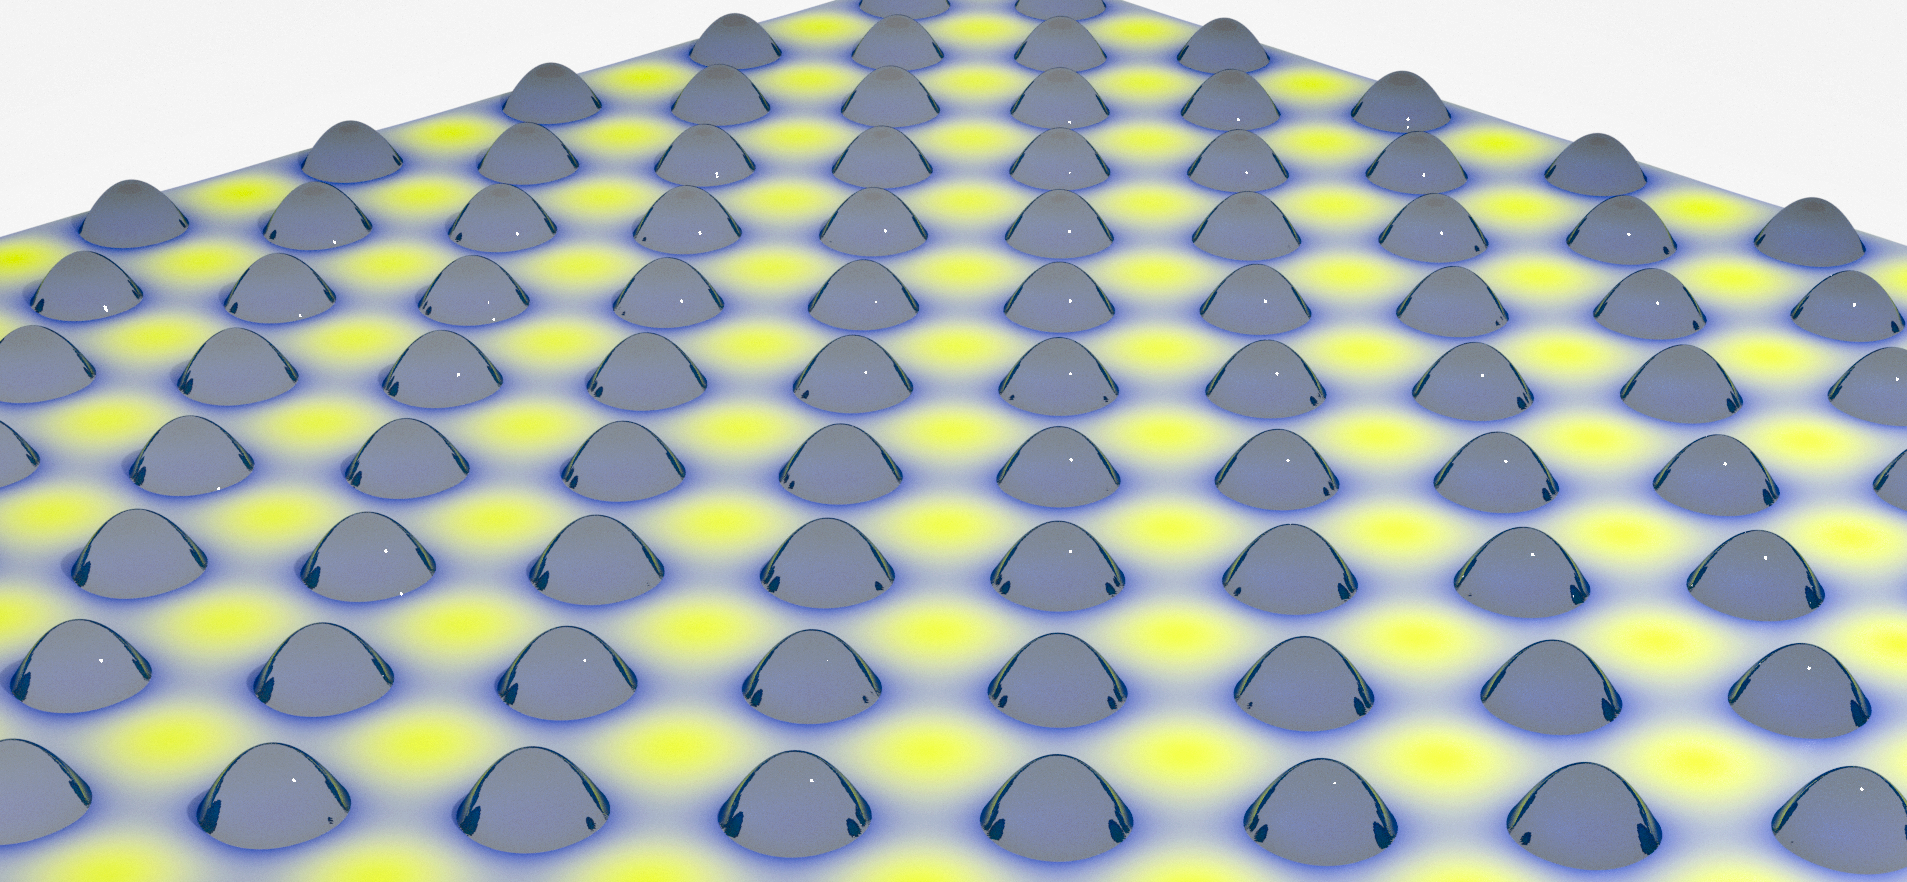
\includegraphics[width=0.4\textwidth]{Figure_1.png}
    \caption{Stationary film thickness field ($t>t_0$) showing the formation of droplets. The color map indicates the contact angle pattern 
    (Eq.~(\ref{eq:sinetheta}) with $v_{\theta}=0$), with lower (higher) values in light blue (yellow).
    }
    \label{fig:handtheta}
\end{figure}
%%%%
Fig.~\ref{fig:handtheta} shows $h(\mathbf{x},t)$ (droplets) and $\theta(\mathbf{x})$ (color coded) for $v_{\theta} = 0$ (i.e. the static case) and \REV{$\lambda = 256 h_0$}~\footnote{For a better visualization double the domain length $L$ and periodically continue the image.}, in late stages of dewetting.
As expected, droplets form in regions of small contact angles (blue) while the regions of high contact angles (yellow) dewet.

\noindent {\it Results.} We first investigate how the rupture times depend on the parameters characterizing the wettability pattern, namely the wavelength of the contact angle variation, $\lambda$, and wave speed, $v_{\theta}$.
The film rupture time, $\tau_r$, is defined as the least $t$ such that $h(\mathbf{x},\tau_r)=h_{\ast}$ (i.e., when the free surface "touches" the substrate).
In Fig.~\ref{fig:model_rt} we report the rupture times as a function of the wavelength, for stationary ($v_{\theta}=0$) and time-dependent ($v_{\theta}=20 v_0$) patterns. 
It is conveyed that, overall, rupture occurs earlier on the static substrate, suggesting that the time variation tends to stabilize the film, in agreement with linear stability analysis results~\cite{suman2006dynamics}.
We observe that $\tau_r$ grows linearly with $\lambda$ for short wavelengths and quadratically for longer $\lambda$.
These facts can be qualitatively explained as follows. 
In this case, from the linearized thin-film equation (in one spatial dimension, for simplicity), obtained setting $h=h_0 + \delta h$ with $\delta h \ll h_0$, 
we can easily see that the exponential growth of the height perturbation is affected by the wettability pattern (variable contact angle) in such a way that $\partial_t (\delta h) \propto (\partial_x^2 (\partial_h\Pi(h_0))) \delta h$. Therefore, since the characteristic time $t_{\theta}$ can be estimated dimensionally as $t_{\theta} \sim \delta h/\dot{(\delta h)}$, the rupture time should go as
\begin{multline}\label{eq:taur_l2}
    \tau_r \sim t_{\theta} \sim  \delta h/\dot{(\delta h)} \propto \frac{3\mu}{h_0^3}(\partial_x^2 (\partial_h\Pi (h_0)))^{-1} \sim \\
    t_0 \left(\frac{q_{\theta}}{q_0}\right)^{-2} \propto t_0 q_0^2 \lambda^2.
\end{multline}
Conversely, for fast growths ($t_{\theta} \ll t_R$), retraction dominates and fixes the time scale, $\tau_r \sim t_R$. 
The latter is related to the time the liquid takes to flow out of regions of high contact angle, whose size is $\sim \lambda$. Hence we have 
 %\tau_r \sim \tau_R \propto \frac{1}{U_{\Theta}}\lambda,
\begin{equation}\label{eq:taur_l1}
 \tau_r \sim \tau_R \propto U_{\Theta}^{-1}\lambda,
\end{equation}
where $U_{\Theta}$ is the retraction speed $U_{\Theta} = \frac{\gamma \Theta^3}{9\mu}$~\cite{Edwards2016}, with $\Theta = \max_{\mathbf{x}}\theta(\mathbf{x})$.
\begin{figure}
    \centering
    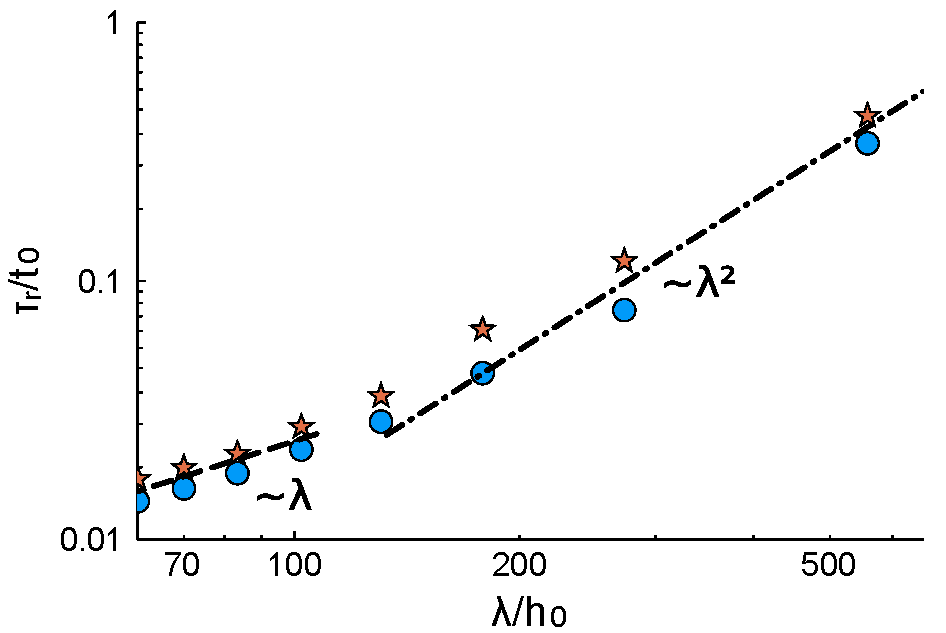
\includegraphics[width=0.4\textwidth]{Figure_2.pdf}
    \caption{Rupture times, $\tau_r$, as a function of the pattern wavelength $\lambda$, for $v_{\theta}=0$ (\textcolor{jlblue}{$\bullet$}) and $v_{\theta}=20 v_0$ 
    (\textcolor{jlorange}{$\star$}).
    The continuous and dashed lines indicate the linear, $\sim \lambda$, and quadratic, $\sim \lambda^2$, scaling laws, respectively.
        }
    \label{fig:model_rt}
\end{figure}
We now focus on the long time dynamics, the characterization of the dewetting morphologies and how they are affected by the speed of the wettability wave.
\begin{figure}
    \centering
    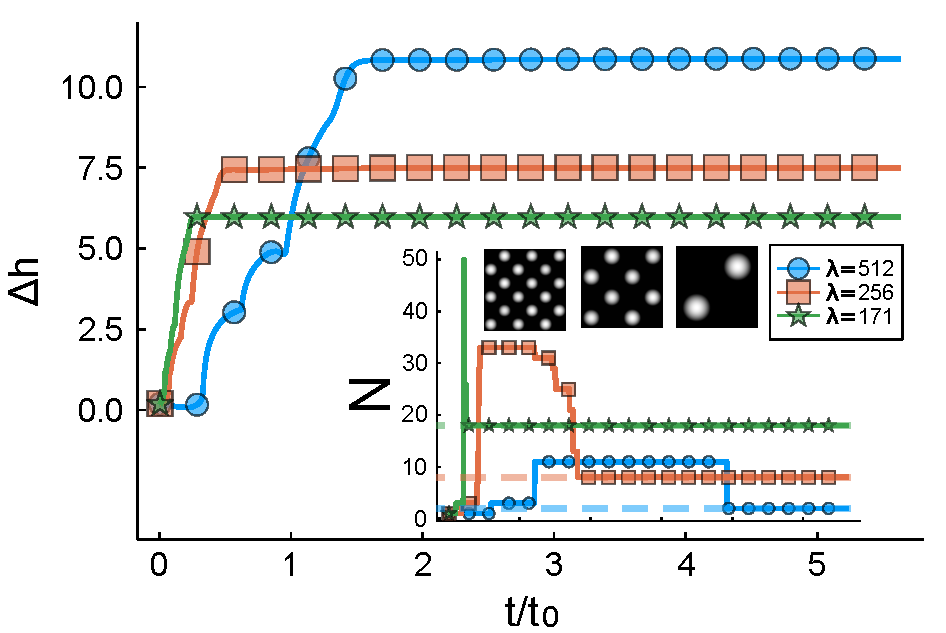
\includegraphics[width=0.4\textwidth]{Figure_3.pdf}
    \caption{MAIN PANEL: Time evolution of the height fluctuations, $\Delta h(t)$, during the dewetting process on the patterned substrate given by       
    Eq.~(\ref{eq:sinetheta})
    with $v_{\theta}= 0$ and $\lambda= 512 h_0$ (\textcolor{jlblue}{$\bullet$}), $\lambda=256 h_0$ (\textcolor{jlorange}{$\blacksquare$}) and $\lambda=170 h_0$ (\textcolor{jlgreen}{$\star$}).
    % The dashed lines indicate the geometrically expected values of the droplet height $h_d$, assuming monodispersity and a perfect spherical cap shape. 
    INSET: Number of droplets, $N(t)$, as a function of time. The three horizontal dashed lines indicate the number of minima of Eq.~(\ref{eq:sinetheta}),
      which is $2\left(\frac{L}{\lambda}\right)^2$. The napshots depict the stationary droplet states as grey-scale images
      of the film thickness field, $h(\mathbf{x},t)$.
      }
    \label{fig:clusters_v0_sine}
\end{figure}
On the stationary substrate, after rupture all fluid accumulates in droplets centered at contact angle minima.
Consequently, as seen from the inset of Fig.~\ref{fig:clusters_v0_sine}, where we plot the number of droplets $N(t)$ vs. time~\footnote{A droplet is identified by the set (``cluster'') of points, in the plane, constituting each of the connected components of the set $\{\mathbf{x} \in [0,L]^2 | h(\mathbf{x},t) \geq h_{\ast}$\}.
% the clusters are determined by means of a Hoshen-Kopelman algorithm~\cite{HK}.
},
in the steady state ($t \gg t_0$) $N(t)$ attains the value $N_{\infty} = 2(L/\lambda)^2$ (horizontal lines), which equals the minima of Eq.~(\ref{eq:sinetheta}), for $v_{\theta}=0$.
Notice that the number of droplets converges faster for smaller pattern wavelengths, in line with the observation reported and justified in the previous section that the characteristic dewetting time decreases with the wavelength.\\
\REV{In the main panel of the figure, the height fluctuations $\Delta h(t) = \max_{\mathbf{x}}\{h(\mathbf{x},t)\}-\min_{\mathbf{x}}\{h(\mathbf{x},t)\}$
grow in time until film rupture and then settle to a constant value. This represents a measure of the mean droplet height $h_d$ (since
droplets are essentially monodisperse), decreasing with the pattern wavelength (as expected, due to a decreasing droplet volume,
$V_d = \frac{h_0 \lambda^2}{2}$).}\\
%In the steady state, since the droplets are essentially monodisperse, this observable . Assuming that the droplet shape is a spherical cap,
%it can be estimated as $h_d =\left(\frac{3V_d(1-\cos(\theta_d))}{\pi(2+\cos(\theta_d))}\right)^{1/3}$, where  is the droplet volume and
%$\theta_d$ is the local contact angle (i.e. the value at the contact line). This, in turn, depends on $h_d$,
%through Eq.~(\ref{eq:sinetheta}), thus making the one above an implicit equation to be solved numerically for $h_d = h_d(\lambda)$. 
%$\Delta h(t)$ is reported in Fig.~\ref{fig:clusters_v0_sine} for three different wavelengths, 
%$\lambda/h_0 = \{170,256,512 \}$, together with the theoretically expected $h_d(\lambda)$ (depicted with lines),
%showing excellent agreement.\\
\begin{figure}
    \centering
    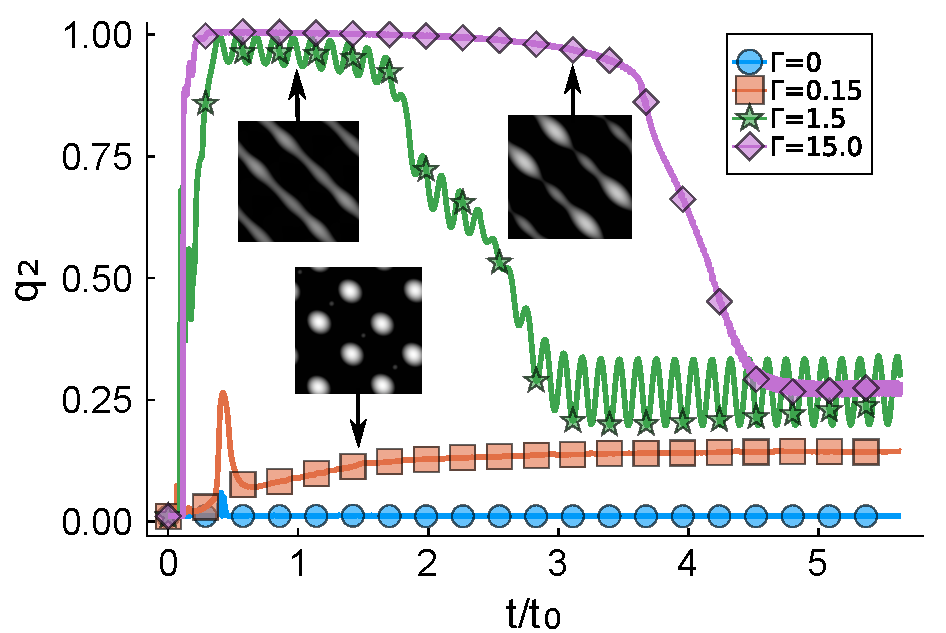
\includegraphics[width=0.4\textwidth]{Figure_4.pdf}
    \caption{Time evolution of the second order Minkowski structure metric, $q_2(t)$, for different $\Gamma$ values, on a substrate with pattern wavelength $\lambda=256 h_0$.
    The grey-scale insets supply snapshots of the corresponding film thickness fields.}
    \label{fig:msm_q2}
\end{figure}
A time-dependent pattern affects the dewetting morphology quite substantially.
For $v_{\theta} = 1.7 v_0$ we still observe the formation of droplets, similarly to the stationary case ($v_{\theta} = 0$). However, these are transported with the contact angle minima, reproducing a somehow similar behaviour recently described in a numerical study of a droplet on a moving wettability step~\cite{GrawitterStark1}.
If the pattern speed is further increased, for $v_{\theta} = 17.5 v_0$ we observe the development of rivulet-like structures, aligned with $\mathbf{v}_{\theta}$. 
The film, in fact, while dewetting in the direction normal to the pattern velocity, is exposed, in the direction of the velocity, to a periodic potential with alternating minima and saddle points, which partially (as we will see) stabilizes the film over ``preferential'' lanes along the diagonals. 
This makes the chosen velocity direction, $(1/\sqrt{2},-1/\sqrt{2})$ (or, equivalently, the orthogonal one $(1/\sqrt{2},1/\sqrt{2})$), optimal for the formation of rivulets. 

In order to better characterize the various morphologies we apply the theory of Minkowski's functionals. 
In particular, we employ the second order Minkowski structure metric, $q_2$~\cite{doi:10.1063/1.4774084, Schaller2020}, which can be computed from a Voronoi tessellation of the set of discrete points $(x_i, y_i)$ on the 2D lattice, such that the height field lies above a certain threshold\footnote{The expression is: $q_2 = \frac{1}{N}\sum_j \frac{1}{P_j}|\sum_k L^{(j)}_k e^{2i\phi^{(j)}_k}|$, where the inner sum runs over the edges of length $L^{(j)}_k$, of the $j$-th Voronoi cell, whose perimeter is $P_j$, and $\phi^{(j)}_k$ is the polar angle of the normal to the $k$-th edge. 
The outer sum represents an ensemble average over the $N$ points in the set.}. The $q_2$ metric quantifies the degree of anisotropy of the dewetting morphology, so it takes relatively large values if the structures formed display a preferential direction. 
Measuring $q_2$ then enables us to clearly distinguish between the formation of droplets and rivulets: much larger $q_2$ values are attained for the latter type of structure, as we can see in Fig.~\ref{fig:msm_q2}.
%Our simulations with $\lambda = L/2$ show a clear difference between $v_{\theta} \leq 0.1v_0$ and $v_{\theta}>0.1v_0$  in $q_2$.
We observe, on the other hand, that such rivulets are metastable and eventually break up into droplets, as indicated by the collapse of $q_2$ at later times. 
Notice, though, that the $q_2$ signal for any $v_{\theta} >0$ always stays above the one for the static case, suggesting that even the smallest pattern velocity introduces a sizeable deformation of the spherical cap shape.
\begin{figure}
    \centering
    % 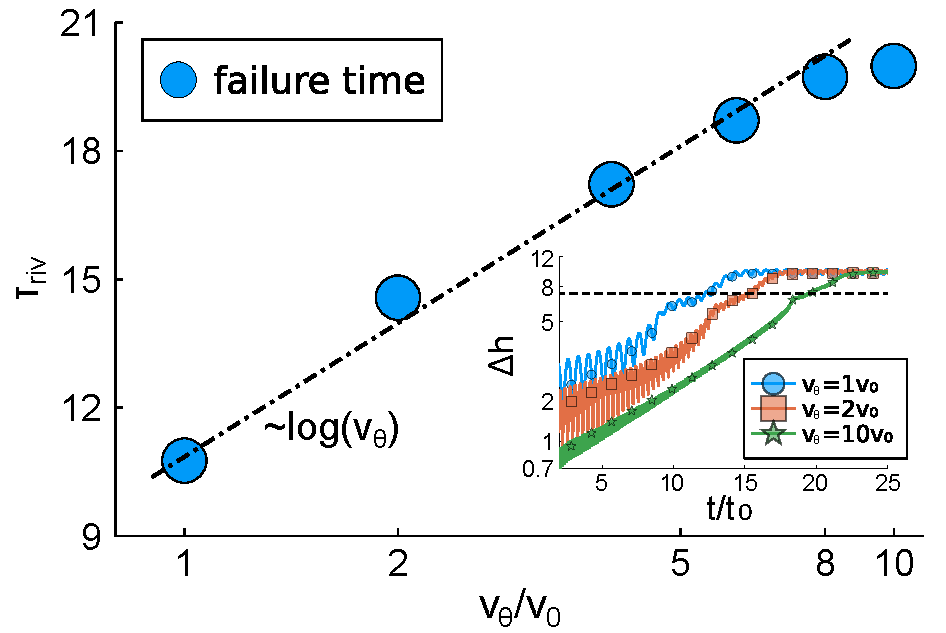
\includegraphics[width=0.45\textwidth]{Figures/Lig_stab_inset_delta_h.pdf}
    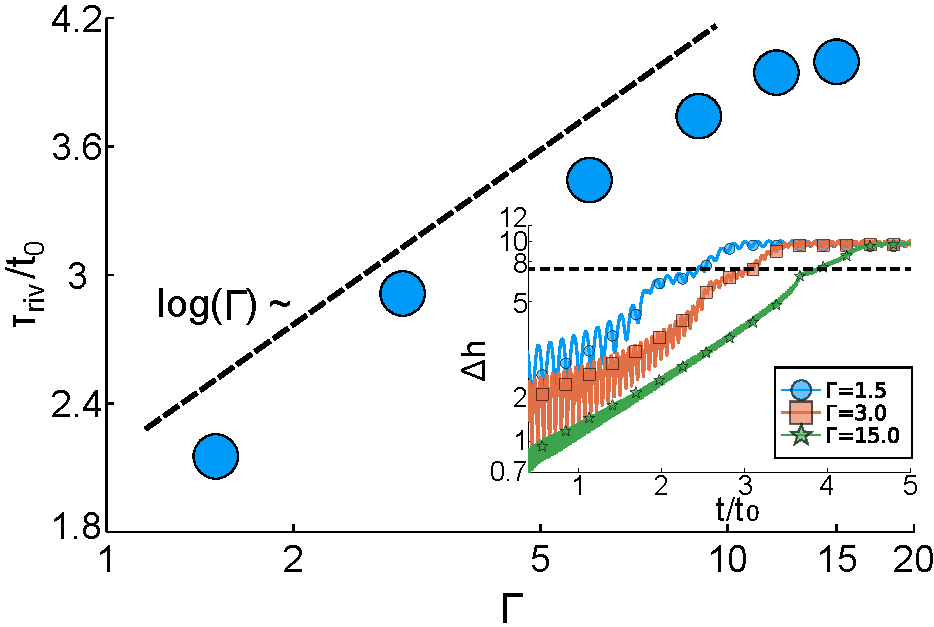
\includegraphics[width=0.4\textwidth]{Figure_5.pdf}
    \caption{MAIN PANEL: Rivulet life-times, $\tau_{\text{riv}}$, for various $\Gamma$.
    The dashed line is a guide to the eye to highlight the logarithmic dependence, in agreement with 
    the theoretical prediction, Eq.~(\ref{eq:rivlt}).
    INSET: Height fluctuations, $\Delta h(t)$, vs time, along the rivulet axis, for three different $\Gamma$.
    }
    \label{fig:stab_ligs_lam2}
\end{figure}
The breakup is the result of a varicose mode of the rivulet~\cite{doi:10.1063/1.3211248, PhysRevE.77.061605}, whose wavelength is $\approx\lambda$, such that only $N_{\infty}/2$ droplets are counted after breakup. 
These droplets show a peculiar dynamics, characterized by a periodic sequence of spreading and retraction, driven by the pattern, that we dub "pumping state"~\footnote{see movie ligament\_formation\_and\_breakup.mp4 in~\cite{SuppMat}.}.

We argue that the emergence of rivulets is controlled by the competition of two characteristic velocities: the pattern wave speed, $v_{\theta}$, and the retraction speed, $U_{\Theta}$, introduced in Eq.~(\ref{eq:taur_l1}). 
\REV{If $U_{\Theta}$ is large as compared to $v_{\theta}$, the film retraction is faster than 
the local contact angle variation and thus droplets form.}
%the transport due to the contact angle field and thus droplets from. 
However, if $v_{\theta}$ is larger than $U_{\Theta}$, then the retracting film has too little time to form droplets and ends up in the metastable rivulet state. \REV{It appears, therefore, natural to consider the ratio of these two velocities, 
$\Gamma \equiv v_{\theta}/U_{\theta}$, as the discriminating parameter.}
%Recalling the expression (\ref{eq:t0}) for the reference velocity $v_0$, %we define the parameter 
%\begin{equation}\label{eq:vel_ratio}
%    \Gamma = \frac{v_{\theta}}{U_{\Theta}} = \frac{3\lambda h_0^3 %q_0^4}{\Theta^3}\chi 
%\end{equation}
%as the ratio of these two velocities,
%where $\chi \equiv v_{\theta}/v_0$. 
We see from Fig.~\ref{fig:msm_q2} that indeed rivulets form only for $\Gamma > 1$. 
Moreover, the larger $\Gamma$, the more stable the rivulets are; in other words, the rivulet life-time, $\tau_{\text{riv}}$, that can be conventionally taken as the time at which the drop of $q_2$ occurs, grows with $v_{\theta}$ (see Fig.~\ref{fig:stab_ligs_lam2}).
The rivulet itself is, in fact, prone to dewetting, with the liquid accumulating over patches around contact angle minima. However, as the pattern moves, the instability is tamed due to configurations whereby higher contact angle regions underlie height field maxima, thus tending to revert the fluid flow.
Heuristically speaking, this means that, if we evaluate $\Delta h(t)$ restricted on the rivulet axis, it should grow exponentially (with a certain growth rate $\alpha \propto t_0$) only when the system is in the unstable configuration. Namely, $\Delta h(t)/\Delta h_0 \propto e^{\alpha t}$ (see inset of Fig.~\ref{fig:stab_ligs_lam2}) with a prefactor proportional to the time spent by the rivulet in such a configuration, which goes as $\sim \lambda/v_{\theta}$, therefore 
$\Delta h(t)/\Delta h_0 \sim \alpha (\lambda/v_{\theta})e^{\alpha t}$. 
The rivulet life-time can be seen as the rupture time of the structure along its axis, hence such that $\Delta h (\tau_{\text{riv}}) \sim h_0$~\cite{PhysRevE.104.034801}, which yields
\begin{equation}\label{eq:rivlt}
    \tau_{\text{riv}} \sim \alpha \log(v_{\theta}) \propto t_0 \log(\Gamma). 
\end{equation}
This logarithmic dependence is indeed observed in the numerical data as shown in Fig.~\ref{fig:stab_ligs_lam2}.\\
\REV{We envisage a possible realization of a 
dewetting experiment on a switchable substrate of the type modeled by the spatio-temporal 
contact angle (\ref{eq:sinetheta}). One may think of a thin liquid film cast on a light responsive substrate~\cite{IchimuraEtAl_Science2000}, under the action of controlled 
external stimuli (a light emitter). 
An ideal candidate could be a digital multimirror device (DMD).
This technology was effectively used for thin film experiments and additive manufacturing~\cite{doi:10.1021/jp301092y, doi:10.1126/science.aax8760}. It allows for fast temporal modulations of the optical signal (with frequencies up to $\approx 16 \, \text{kHz}$)
with spatial resolution of $\approx 10 \times 10 \, \mu \text{m}^2$ (the size of a pixel).
Considering as a reference, for instance, the system studied in~\cite{becker2003complex,PhysRevLett.99.114503}, namely a $\sim 4 \, \text{nm}$ thick film 
of polystyrene deposited on an oxidized silicon wafer,  
we evaluate the retraction speed 
$U_{\Theta} = \frac{\Theta^3 \gamma}{9 \mu}$ to be 
$U_{\Theta} \approx 10^{-2} \, \mu \text{m}/\text{s}$. 
The (minimum) {\it pattern speed} can be 
estimated from the pixel size with frame rate $\sim 1 s^{-1}$ as 
$v_{\theta} \sim 10 \, \mu \text{m}/\text{s}$, which  would result in $\Gamma \sim 10^3$, i.e. well within the rivulet regime ($\Gamma > 1$). Also, both $U_{\Theta}$ and $v_{\theta}$ can be widely modulated: the former by varying the (temperature and molecular weight dependent) viscosity 
or tailoring the substrate to make it more hydrophobic (i.e. increasing the contact angle); the latter, by tuning
the spatial resolution and frame rate of the DMD. Thus, we expect the range of achievable $\Gamma$'s to 
be feasibly extended both to very high ($\Gamma \gg 1$) and very low ($\Gamma \ll 1$) values.}\\
\noindent {\it Conclusions.}
We presented numerical simulations and a theoretical analysis on the dewetting of thin liquid films on a switchable substrate, modelled with a space and time periodically varying contact angle in the thin-film equation.
Studying how the film stability depends on the underlying static pattern, we found that the rupture times grow linearly with the pattern wavelength, for short wavelengths, and quadratically in the long wavelength limit. 
In the time-dependent case, the rupture times are generally longer, indicating an induced greater film stability, and, while the quadratic growth is preserved at long wavelengths, a plateauing behavior was observed as the wavelength decreases. 
A theoretical explanation was provided for all these regimes.
Furthermore, we showed that, at increasing the wettability wave speed, a transition occurs in the dewetting morphology from a multi-droplet to a metastable multi-rivulet state. 
A dimensionless parameter, $\Gamma$, controlling the transition was identified in the ratio of the pattern speed and the typical film retraction speed. 
The rivulets life-time itself grows with the pattern speed, displaying a logarithmic dependence that was captured by means of phenomenological arguments.
On a broader perspective, our work suggests that switchable substrates offer a new avenue to control thin film dewetting, with obviously relevant implications, for instance, for open microfluidic devices, and paves the way to future studies in this direction, exploiting more complex and dedicated space-time dependencies.

\noindent {\it Acknowledgements}. We acknowledge financial support from the German Research Foundation (DFG) (priority program SPP2171 / project HA-4382/11 and Project-ID 431791331—CRC1452), and from the Independent Research Fund Denmark (grant 9063-00018B). 

\bibliography{Ref}

\end{document}
